


\section{Question 1}
\label{part1}

Write a program that extracts 10000 tweets with links from Twitter. 
	Reference - http://thomassileo.com/blog/2013/01/25/using-twitter-rest-api-v1-dot-1-with-python/ 
	Other resources are available 
	Note that only Twitter API 1.1 is currently available; version 1 code will no longer work. 
	
\begin{itemize}
\item Save the tweets URIs, and the mapping to the link(s) each tweet contains 
\item For each \url{t.co} link use ``curl –I –L'' to record the HTTP headers all the way to a terminal HTTP status (i.e. chase down all the redirects)
\item How many unique final URIs? How many duplicate URIs?
\item Build a histogram of how many redirects (every URI will have at least 1) \url {http://en.wikipedia.org/wiki/Histogram}
Build a histogram of HTTP status codes encountered (you’ll have at least 20000: 10000 301s, and 10000+ more)
\end{itemize}
\subsection{Solution}

The following steps were taken to extract tweets from twitter:
\begin{itemize}
	\item Consumer key,Consumer secret key,OAUTH token,OAUTH secret token are collected by registering an Application 
	in Twitter with an account.
	\item Tweepy Package is used to get the URI's from tweets for a specific keyword.
	\item Tweet Id,Tweet URI,Tweet Created Date are stored in file as json format for further usage.
	\item Requests package is used to get all redirect headers,redirect count and final URI's.
	\item Unique URI's ,Duplicate URI's are counted using set function in python.
\end{itemize}
\newpage
\subsection{Code Listing}
Here is the python code that is used to collect Thousand URL's from twitter. 


\lstinputlisting[language=Python,breaklines = true,frame=single,caption={Python program for extracting 10000 links for a given keyword}, label=lst:q1-1,captionpos=b,numbers=left,showspaces=false,showstringspaces=false,basicstyle=\footnotesize]{TweepySearch.py}
\newpage

\subsubsection{histogramData.py}
\lstinputlisting[language=Python,breaklines = true,frame=single,caption={Python program to find count of unique,duplicate final URI's and }, label=lst:q1-2,captionpos=b,numbers=left,showspaces=false,showstringspaces=false,basicstyle=\footnotesize]{histogramData.py}

\subsubsection{Uniqueuris.py}
\lstinputlisting[language=Python,breaklines = true,frame=single,caption={Python program to find count of unique,duplicate final URI's and }, label=lst:q1-2,captionpos=b,numbers=left,showspaces=false,showstringspaces=false,basicstyle=\footnotesize]{Uniqueuris.py}
\newpage
\subsubsection{RedirectHistogram.R}
\lstinputlisting[language=Python,breaklines = true,frame=single,caption={R program for creating histogram to represent redirect frequency of URI }, label=lst:q1-3,captionpos=b,numbers=left,showspaces=false,showstringspaces=false,basicstyle=\footnotesize]{RedirectHistogram.R}

\subsubsection{StatusCodesHistogram.R}
\lstinputlisting[language=Python,breaklines = true,frame=single,caption={R program for creating histogram to represent status codes frequency of URI}, label=lst:q1-4,captionpos=b,numbers=left,showspaces=false,showstringspaces=false,basicstyle=\footnotesize]{StatusCodesHistogram.R}
\newpage
\subsection{Results}


\lstinputlisting[language=Python,breaklines = true,frame=single,caption={Sample Result for Above Program}, label=lst:q1-1,captionpos=b,numbers=none,showspaces=false,showstringspaces=false,basicstyle=\footnotesize]{SampleResult.txt}


\begin{figure}[ht]    
    \begin{center}
        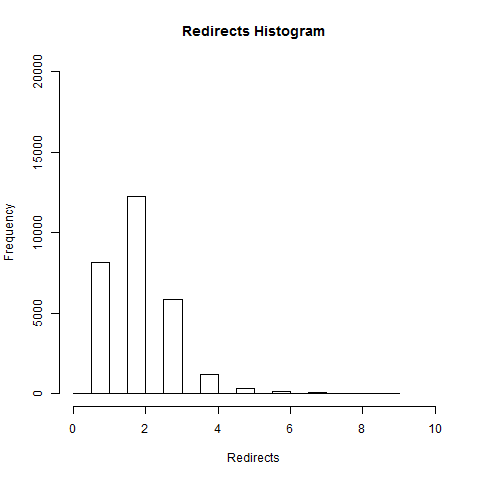
\includegraphics[scale=0.60]{Redirecthistogram.png}
        \caption{Histogram}
        \label{RedirectHistogram}
    \end{center}
\end{figure}

\begin{figure}[ht]    
    \begin{center}
        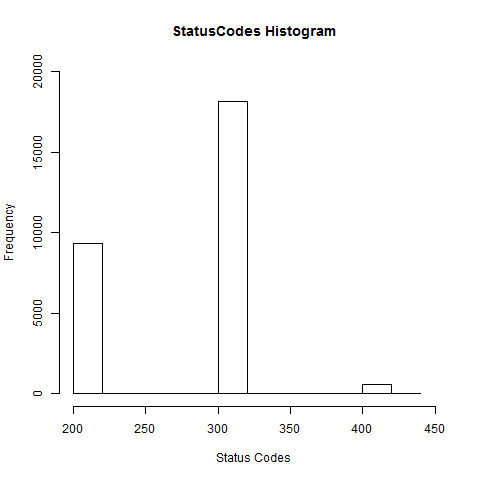
\includegraphics[scale=0.60]{StatusCodeshistogram.png}
        \caption{Histogram}
        \label{StatusCodesHistogram}
    \end{center}
\end{figure}